\documentclass{standalone}
\usepackage{pgf}
\usepackage{tikz}
\usepackage{amsmath,amssymb}
%matrix
\newcommand{\mt}[1]{\ensuremath{\mathbf{#1}}}
%vector
\newcommand{\vc}[1]{\ensuremath{\boldsymbol{#1}}}
%set
\newcommand{\st}[1]{\ensuremath{\mathcal{#1}}}
%time index
\newcommand{\tm}[1]{\ensuremath{\sp{(#1)}}}


%x
\newcommand{\x}[0]{\ensuremath{\vc{x}}}
%s
\newcommand{\s}[0]{\ensuremath{\vc{s}}}
%W
\newcommand{\W}[0]{\ensuremath{\mt{W}}}



\usetikzlibrary{arrows,automata,matrix}
\usepackage[latin1]{inputenc}
\begin{document}


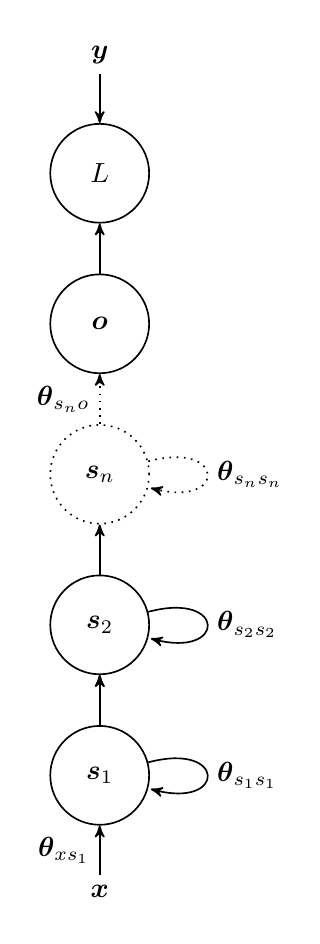
\begin{tikzpicture}[->,>=stealth'
  ,shorten >=0pt
  ,auto,node distance=2.8cm,
  semithick]
  \tikzstyle{every state}
  =[minimum size={10pt+width("$x^{(t-1)}$")}]

  \matrix (m) [matrix of nodes
  ,row sep=.25in,column sep=.25in] {
    \node[     ](y) {$\vc{y}$}; \\
    \node[state](L) {$L$}; \\
    \node[state](o) {$\vc{o}$}; \\
    \node[state,dotted](sn) {$\vc{s}_n$}; \\
    \node[state](s2) {$\vc{s}_2$}; \\
    \node[state](s1) {$\vc{s}_1$}; \\
    \node[     ](x) {$\vc{x}$}; \\
  };

  \path
  (x)  edge  node             {$\vc{\theta}_{xs_1}$}  (s1)
  (s1) edge [loop right] node {$\vc{\theta}_{s_1s_1}$} (s1)
  (s2) edge [loop right] node {$\vc{\theta}_{s_2s_2}$} (s2)
  (s1) edge  node {}                                 (s2)
  (s1) edge  node {}                                 (s2)
  (s2) edge  node {}                                 (sn)
  (o)  edge  node {}                                 (L)
  (y)  edge  node {}                                 (L)
  ;
  \path [dotted] 
  (sn) edge  node {$\vc{\theta}_{s_no}$}               (o)
  (sn) edge [loop right] node {$\vc{\theta}_{s_ns_n}$} (sn)
  ;
  
\end{tikzpicture}

\end{document}